%\chapter{det-comp}


%%%%%%%%%%%%%%%%%%%%%%%%%%%%%%%%%%%%%%%%%%%%%%
\section{Anode Plane Assemblies}

The current baseline for the protoDUNE single-phase TPC is a double-sided structure consisting of wires that wrap in a helical pattern around the length of the APA frame.  All wires eventually terminate on the short end of the APA frame, with electronic readout of all channels located on only one end, thus enabling the APAs to be ``tiled" into a plane within the cryostat.  



\subsection{Scope, requirements, design parameters (Mitch and Bo)}

Figure \ref{fig:tpc_apa1} depicts a protoDUNE APA.  Each side of a double-sided APA consists of four layers of anode wires, plus an additional mesh layer that serves to shield the anode planes from pickup from the Photon Detection System and also from ``ghost" tracks created when ionizing particles have a trajectory that passes through the anode planes.  

\begin{cdrfigure}[APA Diagram]{tpc_apa1}{Sketch of a protoDUNE APA.  Each APA features a Collection plane (blue wires) on both sides, as well as Induction planes (purple and green) that have wires continuously ``wrapped" around the frame.}
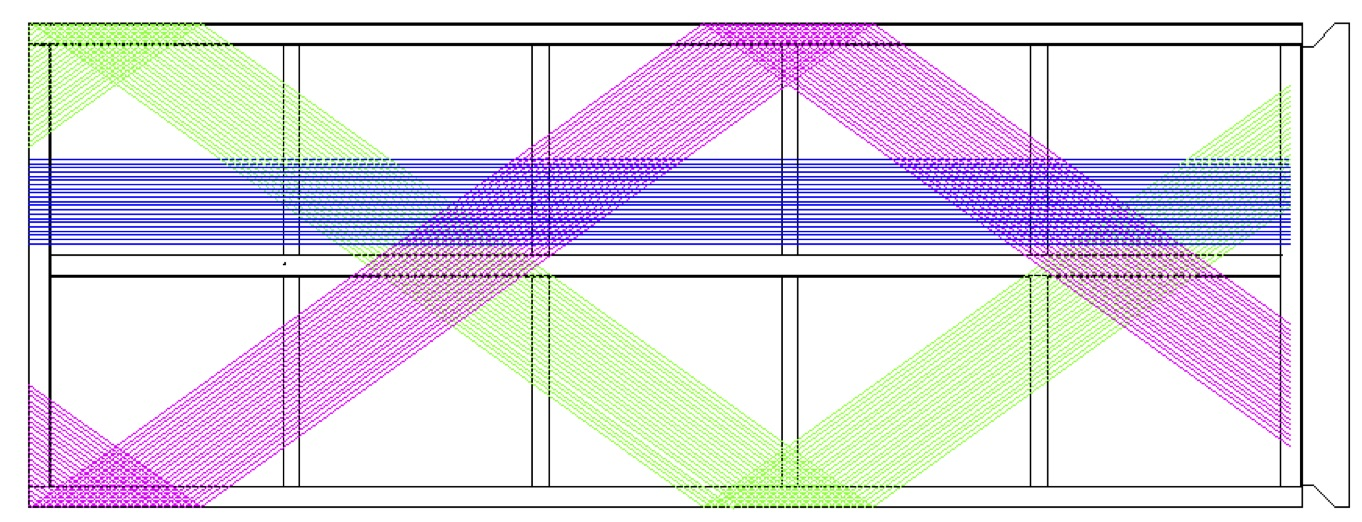
\includegraphics[width=0.5\textwidth, angle=90]{figures/tpc_apa1.jpg} 
\end{cdrfigure}

\subsubsection{Requirements - listing of basic physics requirements.}

\subsubsection{Overall physical description - connection to requirements.}
\begin{itemize}
\item{Size}
\item{Wire spacing}
\item{Plane spacing}
\item{Number of channels}
\item{Angle and reason for chosen angle}
\item{Wire placement accuracy}
\begin{itemize}
\item{Wire Tension}
\item{Double anchor at each wire end}
\item{Need for intermediate support}
\begin{itemize}
\item{Sag prevention}
\item{Break mitigation}
\end{itemize}
\end{itemize}
\item{Bias, and description of plane purposes (grid, induction, collection}
\item{Voltage requirements for induction plane transparency.}
\item{Frame distortion consequences - (Lee G. will update previous study)}
\item{Trapped volume and bubbles}
\item{Mesh, reasons for mesh}
\item{Grounding - (based on input from EE and grounding/shielding group)}
\end{itemize}

The APA layers are listed in Table \ref{tab:bias}, along with their operating voltages.  The arrangement, from the outside-in, is G-U-V-X-M.  The grid layer is present for pulse-shaping purposes, and is not connected for electronics readout.

\begin{cdrtable}[APA Bias Voltages]{cc}{bias}{Layers within the APA, and baseline bias voltages.  All five of these layers are present on both sides of the APA structure, with the Induction layers connected (``wrapped") electrically across both sides.}   
Anode Plane & Bias Voltage  \\ \toprowrule
Grid (G) & -665 V\\ \colhline
Induction (U) & -370 V\\ \colhline
Induction (V) & 0 V\\ \colhline
Collection (X) & 820 V\\ \colhline
Mesh (M) & 0 V\\
\end{cdrtable}


\subsection{APA physical description, Meeting requirements, Fabrication}
\subsubsection{Wires (Lee)}
\begin{itemize}
\item{Physical description (composition, size, conductivity)}
\item{Yield and break strength}
\item{Target tension and limits to variation from target}
\item{Thermal expansion coefficient}
\begin{itemize}
\item{Similar to stainless steel}
\item{Small wires cool and warm faster than frame - tension ramifications}
\end{itemize} 
\end{itemize}

\subsubsection{APA Frame (Lee)}
\begin{itemize}
\item{Physical shape and dimensions}
\item{Welded vs. modular choice and reason for choosing modular}
\item{Wire loads on frames and ability to withstand these loads}
\item{FEA}
\begin{itemize}
\item{APA hanging from TPC support}
\item{APA simply supported at ends - laid flat}
\item{APA in interface frame - laid flat}
\item{APA in interface frame - landscape position}
\end{itemize}
\item{Reasons that buckling from wire loads is not a concern}
\begin{itemize}
\item{Wires stay in plane of APA frame}
\item{Tension drops quickly with deflection - unlike buckling conditions}
\item{Tension on opposing side increases because of board offset, i.e. - huge counter moment develops with start of deflection}
\end{itemize}
\item{Handling of frame during winding and installation}
\end{itemize}

\subsubsection{Wire and Wire Wrapping (Lee)}
\begin{itemize}
\item{Geometry - for reference}
\item{Wire start and end locations}
\item{Number of channels per plane and per APA - total number of wires and wire segments.}
\item{Side and foot boards - tooth geometry - molded tooth strips.}
\item{Solder and glue}
\begin{itemize}
\item{Proposed methods}
\item{Tests on shorts and long term strength of glue/solder bonds}
\end{itemize}
\item{Mesh description and application equipment}
\item{Head electronics boards}
\item{Modular electronics concept}
\begin{itemize}
\item{Reasons for}
\item{Implementation}
\end{itemize}
\end{itemize}

\subsubsection{Wire supports on inner frame members - combs (Lee)}
\begin{itemize}
\item{Reasons for}
\item{Geometry and appearance}
\item{Installation method}
\item{Tests results concerning wire wear from these supports}
\end{itemize}


\subsubsection{APA Interconnect Features (Lee)}


\subsubsection{Integration with TPC (Dan/Jack)}

\subsection{Wire-winding Machines (Dan)}

\subsubsection{Wire wrapping concept}

\subsubsection{Design requirements}

\subsubsection{Implementation}
\begin{itemize}
\item{Interface frames}
\item{Fixed APA vs. rotating APA}
\item{Tensioning head passed around frame}
\item{Half a layer wrapped before moving APA supports}
\end{itemize}

\subsubsection{Intermittent stop to solder}

\subsubsection{Wire wrapping machinery}

\subsubsection{Description/photos of machinery under construction and test}

\subsubsection{Assembly sequence}

\subsection{QC Procedures}

\subsubsection{Quality documents (Bob, Mike Z.)}

\begin{itemize}
\item{Material certs}
\item{Incoming inspection}
\item{Assembly travelers}
\end{itemize}

\subsubsection{Test plan}

\begin{itemize}
\item{Wire tension}
\end{itemize}

\subsubsection{Assembly procedure (Lee or Dan)}

